\chapter{Introducción}
 En este capítulo se detalla la motivación que llevó a la realización del proyecto, los objetivos que este comprende y las pautas que se tomaron para lograr llevarlo a cabo
    
    \section{Objetivo}
    
    Este Trabajo de Final de Grado busca la implementación de un portal web sencillo y compacto que permita la recopilación de datos de interés para el estudio por parte del equipo médico. Para ello contará con formularios personalizados con los campos de interés  solicitados por el mismo que serán rellenados por los médicos en consultas rutinarias con los pacientes que hayan consentido participar en el proyecto. Estos datos serán luego accesibles tanto vía web como en archivos de excel descargables desde el propio portal.\newline

	Con el fin de ajustar el producto final a las necesidades del equipo la aplicación se entregará con tiempo suficiente (meses de antelación) para que pueda ser probada, revisada y modificada a medida. Esto es especialmente importante ya que el estudio se extenderá muchos meses más allá de la finalización de este TFG.\newline

	El objetivo final, y por supuesto el más importante, es que todo este desarrollo sirva de herramienta para ajustar los criterios de evaluación en los pacientes con diabetes mellitus tipo 2, permitiendo encontrar pautas en sus estados de salud subsanables que puedan en un futuro prevenir más casos de esta enfermedad.\newpage
	
	\section{Motivación}
    
    Nuestra primera motivación para adentrarnos en este proyecto son las tecnologías empleadas en el mismo. Ambos participantes están interesados en centrar su carrera en tecnologías web, uno de ellos trabajando ya de hecho como desarrollador full-stack. El proyecto da además libertad para ser implementado sin ningún tipo de restricciones de diseño o rendimiento, lo que plantea un escenario ideal para experimentar durante su desarrollo.\newline

	El otro motivo principal para decantarnos por este proyecto es su cercanía a un proyecto real. El cliente, la aplicación, los plazos y las necesidades del mismo no son algo creado para un ambiente académico, como otros desarrollos ya efectuados durante la carrera, sino un problema real que precisa una solución realista contando con todas las personas que lo acabarán utilizando. Además el proyecto requerirá de un mantenimiento post entrega, otro ámbito nunca explorado en la carrera que será una valiosa experiencia de cara a nuestro futuro.\newline

	Por último remarcar que uno de los miembros, Sergio, ya tiene buenas experiencias con un proyecto anterior para el ámbito médico desarrollado en solitario para una empresa en Suiza y Eduardo siempre ha tenido interés en los hábitos de vida saludables y la nutrición, posible principal remedio para la diabetes extraído de los resultados de este estudio.\newpage
	
	\section{Metodología de trabajo}
    
    El proyecto será planificado bajo los estándares de la metodología Scrum aunque distendiendo un poco sus cotas temporales, pues al ser solo dos miembros no es necesario hacer un hincapié tan diario en la organización para mantener el orden. Lo primero será definir cómo mantendremos los tres pilares básicos de la metodología: \textbf{transparencia, inspección y adaptación}.
    
    \subsection{Transparencia}
    Para mantener a ambos miembros al día de cualquier avance o variación en el proceso se empleará la herramienta online de Trello, que nos permitirá ir viendo en tiempo real los mismos. Este será estructurado de la siguiente forma:
    
    \begin{itemize}
    \item Se crearán dos columnas, una con la lista de tareas pendientes para el sprint actual y otra con las tareas actualmente en desarrollo. Además se creará una columna por cada sprint en la que se irán almacenando todas las tareas finalizadas. Cada tarea podrá encapsularse en una o más de estas categorías: despliegue, documentación, front, bug, investigación, modelo de datos, pendiente de resolver (cuestión a espera de la próxima reunión con el tutor), back, varios, resuelto (cuestiones ya solucionadas en anteriores reuniones que quedan como recordatorio). Además cada tarea llevará una o más etiquetas indicando los desarrolladores que han trabajado en ella.\newline
    
     \begin{figure}[h]
    \centering
     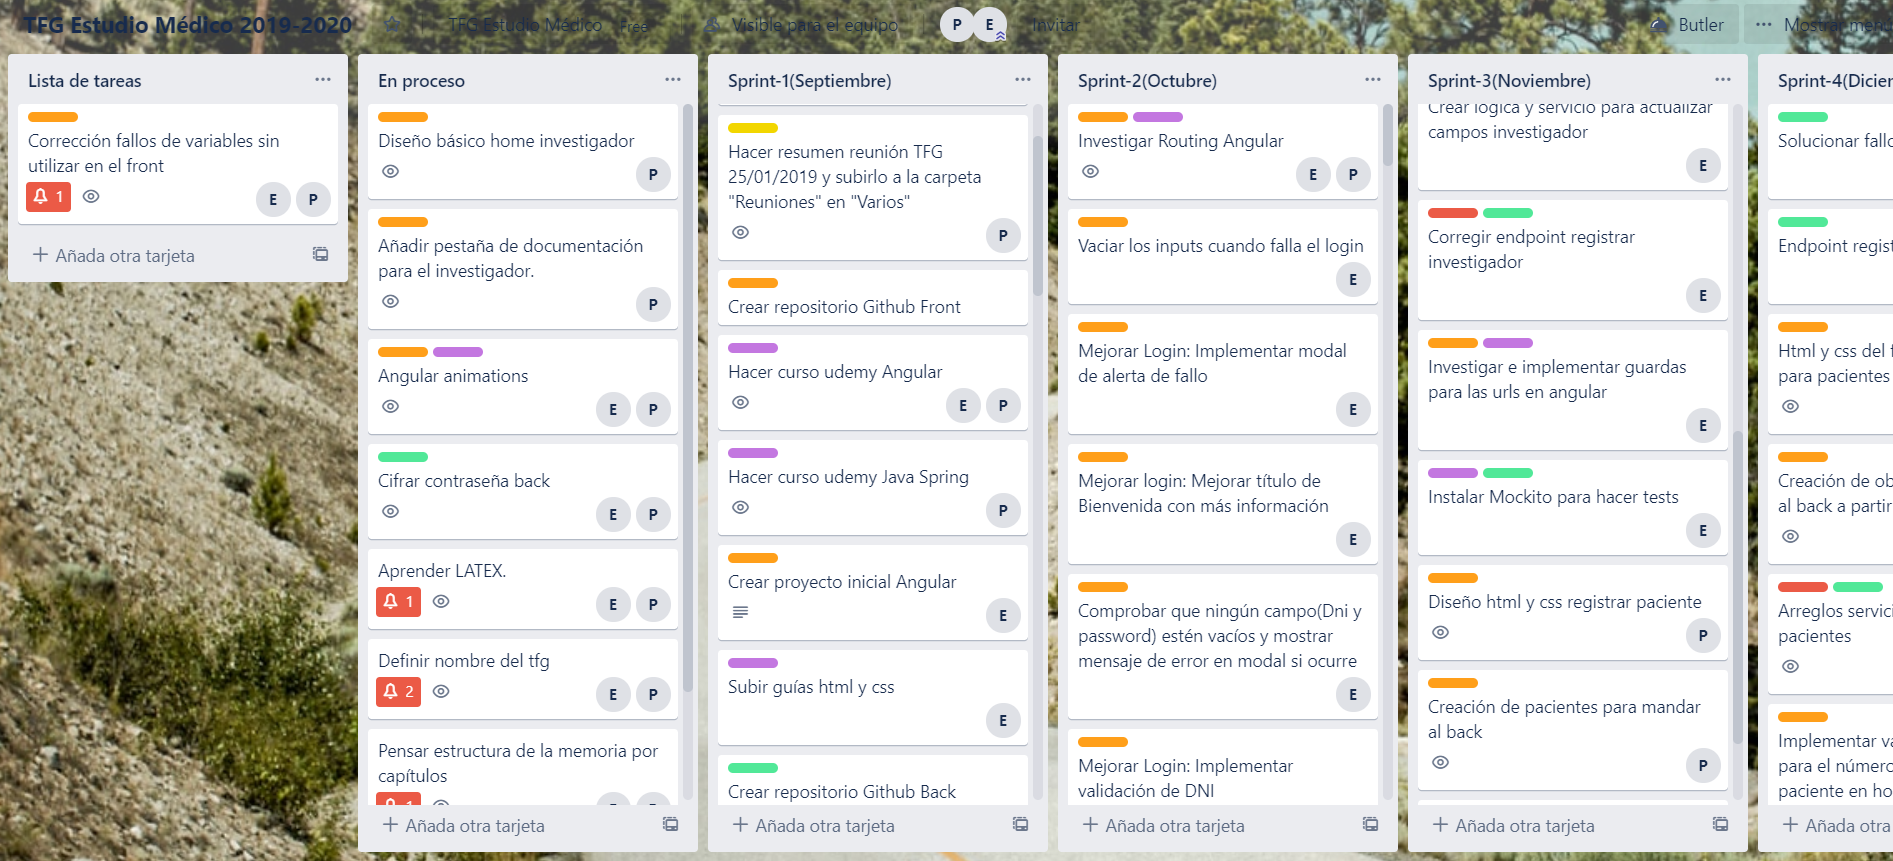
\includegraphics[width=1\textwidth]{images/Trello.jpg}
    \caption{Captura de ejemplo de la herramienta Trello tomada a posteriori.}
    \end{figure}
    \newpage
    
    \item  Además todo el código del proyecto estará subido y actualizado en un repositorio, en este caso GitHub, a traves del cual se podrá ver un histórico preciso de los cambios realizados en cada commit junto a comentarios explicativos del desarrollador que los haya realizado.\newline
    
    \begin{figure}[h]
    \centering
     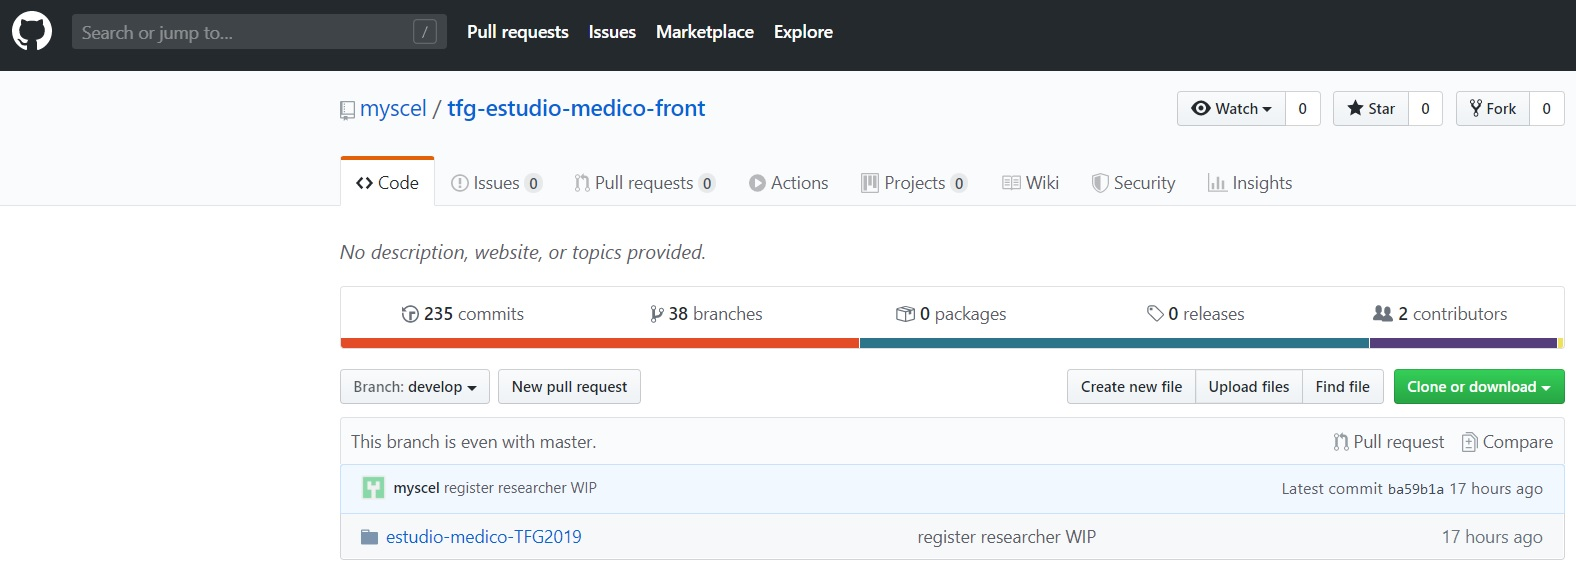
\includegraphics[width=1\textwidth]{images/GitHubFront.jpg}
    \caption{Captura de ejemplo del repositorio front en GitHub tomada a posteriori.}
    \end{figure}
    \end{itemize}
    
    \subsection{Inspección}
    Con el fin de mantener este principio nuestro repositorio no solo albergará código sino también un espacio separado para todos los artefactos derivados de scrum, así como la documentación que se vaya creando durante el proceso que sea relevante a efectos de esta memoria. Estos artefactos serán por tanto accesibles constantemente por ambos miembros, los cuales avisarán en caso de cualquier añadido o modificación para que su compañero pueda revisarlo.\newline
    
    \begin{figure}[h]
    \centering
     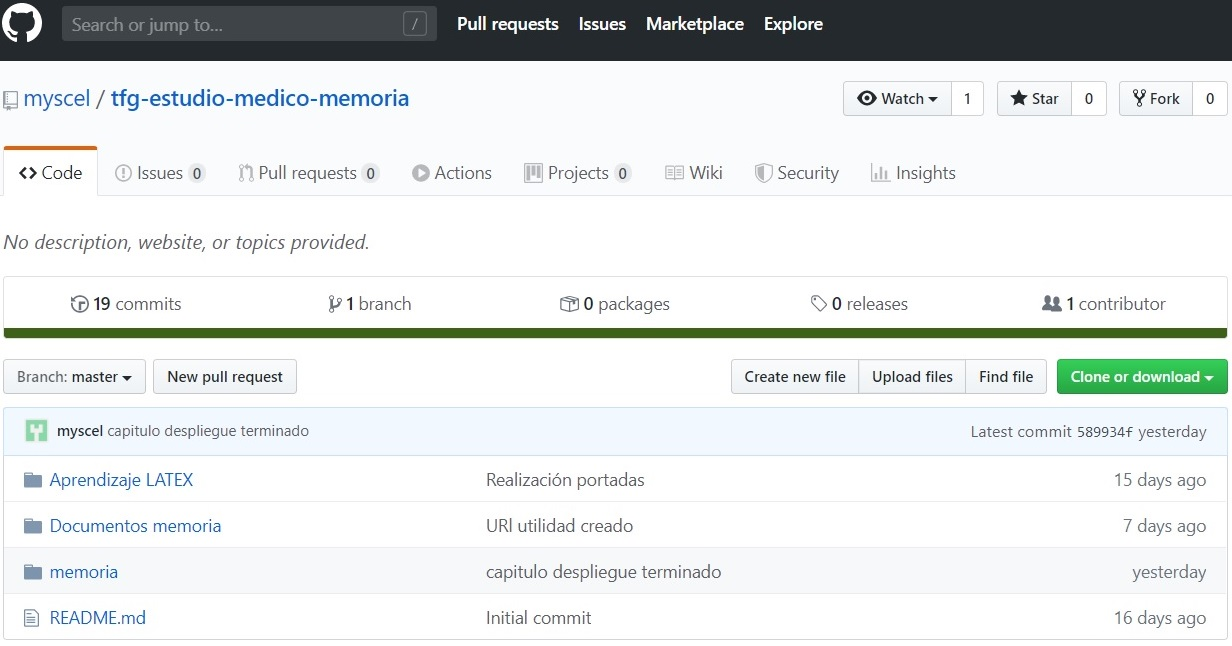
\includegraphics[width=1\textwidth]{images/GitHubMemoria.jpg}
    \caption{Captura de ejemplo del con todos los documentos referentes a la memoria en GitHub tomada a posteriori.}
    \end{figure}
    \newpage
    
     \subsection{Adaptación}
    Al final de cada sprint se realizará una reunión tanto con el tutor del proyecto como con un representante del equipo médico para revisar el proceso y obtener feedback del mismo. Los errores o cambios urgentes extraídos de estas reuniones pasarán a ser la tareas más prioritarias del proyecto y su resolución será notificada de inmediato a ambos asistentes de la reunión. Además para mantener el proyecto lo más afín a las necesidades del cliente cualquier cambio significativo en mitad de un sprint será notificado por correo previamente.
    \newline
    \newline
    \newline
    
    Además de toda la documentación y artefactos mencionados disponibles durante el desarrollo los miembros mantendrán un contacto diario hablando de qué han hecho, qué van a hacer y los problemas que van encontrando, el cual sustituye las Daily Scrum.\newline

	En cuanto a los roles típicos de Scrum en nuestro caso no serán utilizados. El Producto Owner será suplido con la comunicación directa y constante  de los miembros con el cliente que asegurara la priorización del valor para este durante el desarrollo. El Scrum Master no será preciso ya que ambos miembros del equipo tienen experiencia utilizando metodologías ágiles, tanto en la carrera con Scrum como fuera en trabajos o proyectos propios. Por tanto solo existirá el equipo de desarrollo y este suplirá las funciones necesarias del resto de roles.\newline

	Los sprints serán de una duración mensual. Se opta por esta cuantía porque al estar uno de los miembros aún con clases y otro trabajando a jornada completa no se estima que en una semana el desarrollo pueda tener un avance suficientemente significativo. Estos sprints se iniciarán con una reunión de planificación con el tutor del proyecto y el representante del equipo médico, estipulando qué se hará y cómo. Así mismo concluirán con otra reunión de misma índole que mostrará una demo funcional al representante y recogerá su feedback, para acto seguido comenzar con la reunión de planificación del siguiente sprint. Se decide aunar así el inicio y final del sprint en una sola reunión para evitar problemas de horarios difíciles de encajar por parte de los cuatro. Tras esta reunión con todos los miembros se realizará una pequeña reunión de retrospectiva solo del equipo de desarrollo para determinar si la metodología de trabajo funciona y qué se podría modificar o añadir.\newline


